%%%%%%%%%%%%%%%%%%%%%%%%%%%%%%%%%%%%%%%%%%%%%%%%%%%%%%%%%%%%%%%%%%%%%%%%%%%%%%
% CS240: Programming in C
% Copyright 2016 Pejman Ghorbanzade <pejman@ghorbanzade.com>
% Creative Commons Attribution-ShareAlike 4.0 International License
% https://github.com/ghorbanzade/UMB-CS240-2016S/blob/master/LICENSE
%%%%%%%%%%%%%%%%%%%%%%%%%%%%%%%%%%%%%%%%%%%%%%%%%%%%%%%%%%%%%%%%%%%%%%%%%%%%%%

\def \topDirectory {.}
\def \resDirectory {\topDirectory/src/c/main/ls04}
\def \texDirectory {\topDirectory/src/tex}
\def \styDirectory {\texDirectory/sty}
\def \cfgDirectory {\texDirectory/cfg}
\def \imgDirectory {\texDirectory/img}

\documentclass[compress]{beamer}
%\mode<presentation>
%\usetheme{default}

\usepackage{\styDirectory/directives}
%%%%%%%%%%%%%%%%%%%%%%%%%%%%%%%%%%%%%%%%%%%%%%%%%%%%%%%%%%%%%%%%%%%%%%%%%%%%%%
% CS114: Introduction to Programming in Java
% Copyright 2015 Pejman Ghorbanzade <mail@ghorbanzade.com>
% Creative Commons Attribution-ShareAlike 4.0 International License
% https://github.com/ghorbanzade/UMB-CS114-2015F/blob/master/LICENSE
%%%%%%%%%%%%%%%%%%%%%%%%%%%%%%%%%%%%%%%%%%%%%%%%%%%%%%%%%%%%%%%%%%%%%%%%%%%%%%

\course{id}{CS240}
\course{name}{Programming in C}
\course{venue}{Mon/Wed, 5:30 PM - 6:45 PM}
\course{semester}{Spring 2016}
\course{department}{Department of Computer Science}
\course{university}{University of Massachusetts Boston}

\instructor{name}{Pejman Ghorbanzade}
\instructor{title}{}
\instructor{position}{Student Instructor}
\instructor{email}{pejman@cs.umb.edu}
\instructor{phone}{617-287-6419}
\instructor{office}{S-3-124B}
\instructor{office-hours}{Mon/Wed 16:00-17:30}
\instructor{address}{University of Massachusetts Boston, 100 Morrissey Blvd., Boston, MA}

\usepackage{\styDirectory/beamerthemePejman}
\doc{number}{4}
%\setbeamertemplate{footline}[text line]{}

\usepackage{booktabs}

\begin{document}

\prepareCover

\section{Variables}

\begin{slide}
	\begin{block}{Definition}

	A variable is a name for a location in memory used to hold a data value.

	The name of a variable is a sequence of case sensitive letters, digits and the underscore character; the first of which is not a digit.

	\begin{terminal}
	variable_type identifier;
	variable_type identifier = initial_value;
	\end{terminal}

	\end{block}
\end{slide}

\begin{slide}
	\begin{block}{Declaration}

	C is a statically-typed language.
	Type of all variables must be known at compile time.

	A type declaration associates a variable with a type at compile time.

	\begin{terminal}
	int a = 123;
	int b = 99;
	int c = a + b;
	b = 25;
	\end{terminal}

	\end{block}
\end{slide}

\begin{slide}
	\begin{block}{Constants}

	A constant is a special variable that holds a value that may not alter during its lifetime.

	\begin{terminal}
	#define PI 3.14159
	int const PI = 3.14159;
	\end{terminal}

	\end{block}
\end{slide}

\begin{slide}
	\begin{block}{Coding Style Convention}

	\begin{itemize}
	\item[] Avoid long identifiers.
	\item[] Use lowecase for variables.
	\item[] Use uppercase for symbolic constants.
	\item[] Separate words with underscore.
	\end{itemize}

	\end{block}
\end{slide}

\begin{slide}
	\begin{quotation} \scriptsize \normalfont

	C is a Spartan language, and so should your naming be.
	Unlike Modula-2 and Pascal programmers, C programmers do not use cute names like \alert{\texttt{ThisVariableIsATemporaryCounter}}.
	A C programmer would call that variable \alert{\texttt{tmp}}, which is much easier to write, and not the least more difficult to understand.

	[...]

	Local variable names should be short, and to the point.
	If you have some random integer loop counter, it should probably be called \alert{\texttt{i}}.
	Calling it \alert{\texttt{loop\_counter}} is non-productive, if there is no chance of it being mis-understood.
	Similarly, \alert{\texttt{tmp}} can be just about any type of variable that is used to hold a temporary value.

	If you are afraid to mix up your local variable names, you have another problem, which is called the function-growth-hormone-imbalance syndrome.

	\begin{flushright}-- Linux Kernel Coding Style\end{flushright}

	\end{quotation}
\end{slide}

\section{Data Types}

\begin{slide}
	\begin{block}{Definition}

	The type of a variable determines the number of bytes to be assigned to its value and how the bit pattern of its value should be interpreted.

	\begin{terminal}
	int a = 7;
	\end{terminal}

	\end{block}
\end{slide}

\begin{slide}
	\begin{block}{Basic Data Types}

	\begin{columns}
	\column{0.3\textwidth}
	\begin{itemize}
	\item[] int
	\item[] char
	\end{itemize}

	\column{0.4\textwidth}
	\begin{itemize}
	\item[] double
	\item[] float
	\end{itemize}

	\column{0.3\textwidth}
	\begin{itemize}
	\item[] void
	\end{itemize}
	\end{columns}

	\end{block}
\end{slide}

\begin{slide}
	\begin{block}{Signed vs. Unsigned}

	By default, the left-most bit of a variable is reserved to indicate sign of its value.
	If the value of a variable is ensured to be non-negative, it is possible to instruct the compiler not to reserve a \emph{sign} bit.

	\begin{terminal}
	int a;
	unsigned int b;
	\end{terminal}

	\end{block}
\end{slide}

\begin{slide}
	\begin{block}{Integer Data Types}

	You can instruct the compiler to reserve less or more bytes for an integer variable.

	\begin{itemize}
	\item[] short
	\item[] long
	\end{itemize}

	\end{block}
\end{slide}

\begin{slide}
	\begin{block}{Integer Types}

	\begin{table}
	\begin{tabular}{lcc}
	\toprule
	Type & Storage Size & Value Range \\
	\midrule
	char & 1 byte & -128 to 127 \\
	int & 4 bytes & $-2^{32-1}$ to $2^{32-1}$ \\
	short & 2 bytes & -32768 to 32767 \\
	long & 8 bytes & $-2^{64-1}$ to $2^{64-1}$ \\
	\bottomrule
	\end{tabular}
	\end{table}

	\end{block}
\end{slide}

\begin{slide}
	\begin{block}{Floating-Point Types}

	\begin{table}
	\begin{tabular}{lcc}
	\toprule
	Type & Storage Size & Value Range \\
	\midrule
	float & 4 bytes & 1.2E-38to 3.4E+38 \\
	double & 8 bytes & 2.3E-308 to 1.7E+308 \\
	long double & 16 bytes & 3.36E-4932 to 1.19E+4932 \\
	\bottomrule
	\end{tabular}
	\end{table}

	\end{block}
\end{slide}

\begin{slide}
	\begin{block}{Void Type}

	The \alert{void} data type is used to indicate that no value is available.
	It is used in three situations:

	\begin{itemize}
	\item[] To specify type of return value of a function that does not return anything.
	\item[] To specify type of argument of a function that does not accept any argument.
	\item[] To access address of a data object instead of its value.
	\end{itemize}

	\end{block}
\end{slide}

\begin{slide}
	\begin{block}{Note}

	Declared data type should be consistent with the value assigned.

	\inputminted[
		fontsize=\scriptsize,
		firstline=14,
		lastline=19,
		linenos
	]{c}{\resDirectory/hello-cmd1.c}

	\end{block}
\end{slide}

\begin{slide}
	\begin{block}{Remember}

	\begin{itemize}
	\item[] C does not provide a boolean data type.
	\item[] C does not provide a String data type.
	\end{itemize}

	\end{block}
\end{slide}

\begin{slide}
	\begin{figure}
	
\includegraphics[width=0.8\textwidth]{\imgDirectory/boolean.jpg}
	\end{figure}
\end{slide}

\section{Command Line Arguments}

\begin{slide}
	\begin{block}{Definitions}

	Command line arguments are a list of string literals separated by whitespace with which your program is invoked.

	\end{block}
\end{slide}

\begin{slide}
	\begin{block}{Motivation}

	Command line arguments provide efficient interthread communication through piping and redirection.

	\end{block}
\end{slide}

\begin{slide}
	\begin{block}{Implementation}

	\inputminted[
		fontsize=\scriptsize,
		firstline=10,
		linenos
	]{c}{\resDirectory/hello-cmd1.c}

	\end{block}
\end{slide}

\begin{slide}
	\begin{block}{Demonstration}

	\begin{terminal}
	pejman@cs240$ gcc hello-cmd.c -o hello-cmd
	pejman@cs240$ ./hello-cmd CS240
	Hello CS240!
	pejman@cs240$ ./hello-cmd Pejman
	Hello Pejman!
	pejman@cs240$ ./hello-cmd Mr President
	Hello Mr!
	\end{terminal}

	\end{block}
\end{slide}

\begin{slide}
	\begin{block}{Problem Statement}

	A programmer has no prior knowledge of how the program will be executed.

	\begin{terminal}
	pejman@cs240$ gcc hello-cmd.c -o hello-cmd
	pejman@cs240$ ./hello-cmd
	Hello (null)!
	\end{terminal}

	\end{block}
\end{slide}

\begin{slide}
	\begin{block}{Proposed Solution}

	\inputminted[
		fontsize=\scriptsize,
		firstline=10,
		linenos
	]{c}{\resDirectory/hello-cmd2.c}

	\end{block}
\end{slide}

\begin{slide}
	\begin{block}{Notes}

	\begin{itemize}
	\item[] All command line arguments are given before program execution.
	\item[] Each command line argument is an array of character.
	\end{itemize}

	\end{block}
\end{slide}

\begin{slide}
	\begin{figure}
	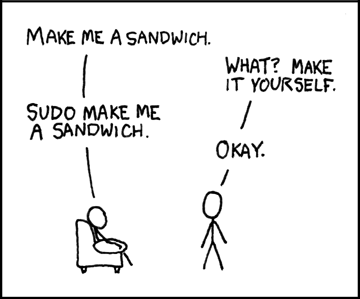
\includegraphics[width=0.6\textwidth]{\imgDirectory/sudo.png}
	\end{figure}
\end{slide}

\end{document}
